
\section*{Introduction}\label{sec:intro}

Rule-based modeling languages for molecular biology, such as Kappa
\cite{DanosEtAl-CONCUR07} and BioNetGen \cite{bngl}, or organic
chemistry, such as M{\o}d \cite{moll}, can be used to write
mechanistic models of complex reaction systems. In these approaches,
chemical transformations are represented by local graph-rewrite rules
equipped with stochastic firing rates. In a dynamical simulation,
rules induce a time series of events that might reach a state of
interest in processes like the assembly of a molecular machine, the
activation of a transcription factor, or the synthesis of a specific
chemical compound. While rule-based models provide compactness,
transparency, and the ability of handling combinatorial complexity,
the perhaps most significant advantage lies in their suitability for
causal analysis that takes into account the logically concurrent
nature of interactions.

The causal analysis
\cite{DBLP:conf/fsttcs/DanosFFHH12,DanosEtAl-CONCUR07} of event series
generated by such models provides a formal definition of ``pathway"
and a means for revealing the emergence of pathways from low-level
interactions. These methods take advantage of rule structure to
\begin{inparaenum}[(i)]
\item compress a given simulation trace into a minimal subset of
  events that are necessary and jointly sufficient to replicate a
  phenomenon of interest and
\item highlight the direct causal influences between events, exposing
  the extent of concurrency.
\end{inparaenum}

% There is much more to discuss here.

We propose a distinct but complementary approach based on
\textit{counterfactual reasoning} that improves causal explanations by
\begin{inparaenum}[(i)]
\item being more sensitive to kinetics and
\item properly accounting for the causal impact from inhibition
  between events.
\end{inparaenum}

\section{Motivating example}\label{sec:example}

% Much more to say about Kappa

We illustrate the need for counterfactual reasoning on a toy example
in Kappa. Consider a model with two types of agents, kinases $K$ and
substrates $S$, interacting according to the rules depicted in
Figure~\ref{fig:model}.

% -*- TeX-master: "ijcai18.tex" -*-

\begin{figure}[h]
  \vskip -0.2cm
  \begin{center}
    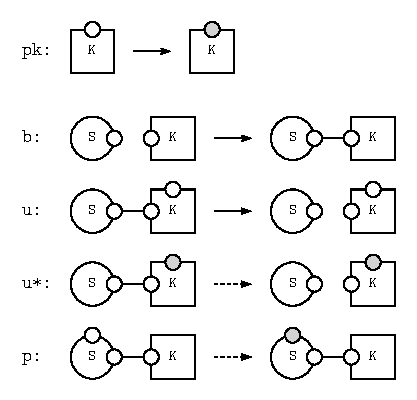
\includegraphics[scale=0.9]{figures/model.pdf}
  \end{center}
  \vskip -0.2cm
  % \caption{A motivating toy model. As usual in Kappa, sites not
  %   mentioned in a rule are left unchanged by it. Instead of naming
  %   sites, we here identify them by their position on an
  %   agent. Phosphorylated sites are shown in gray. Firing rates are
  %   not specified here but dotted arrows indicate \textit{slow}
  %   reactions, whereas solid arrows indicate \textit{fast} reactions.}
  \caption{A motivating toy model. Sites not mentioned in a rule are
    left unchanged by it. \longversion{As in
      Figure~\protect\ref{fig:mixture}, sites are identified by their
      position on an agent.}  Firing rates are not specified, but
    dotted (solid) arrows indicate \textit{slow} (\textit{fast})
    reactions
    $(\lambda_u \gg \lambda_{u^*} \approx \lambda_p)$.}
  \label{fig:model}
\end{figure}


For the sake of simplicity, consider an initial mixture $I$ with only
a single kinase and a single substrate whose sites are free and
unphosphorylated. We then ask: Starting from $I$, \textbf{how} is $p$
triggered ? We are not merely looking for an account of reachability
but rather for causal narratives, that is, collections of necessary
events connected by causal influences.

A stochastic simulation \cite{DanosEtAl-APLAS07} might produce the
following trace (events are labelled by the rules that induced them):
\begin{align}\label{example-trace} b,\ \ u,\ \ pk,\ \ b,\ \ p,\ \
  u^{*},\ \ \cdots
\end{align} Figure~\ref{fig:dumb-story} depicts the causal narrative
explaining the occurrence of $p$ according to existing techniques
\cite{DBLP:conf/fsttcs/DanosFFHH12,DanosEtAl-CONCUR07}. The arrow
between $b$ and $p$ is called an \textit{activation arrow}, meaning
that $b$ modifies an aspect of state (by creating a link) that enables
$p$ to happen.

\begin{figure}[H]
  \vskip -0.8cm
  \begin{center}
    \includegraphics[scale=0.7]{figures/dot/dumb-story.pdf}
  \end{center}
  \vskip -1cm
  \caption{A causal explanation for $p$ in trace
    (\ref{example-trace}).  Events are labelled by the rules that
    induced them. The \emph{init} node corresponds to a special event
    that sets the mixture to its initial state.  }
  \label{fig:dumb-story}
\end{figure}


This narrative, however, is blind to the critical role of $pk$ in the
original trace. Looking at the rules in Figure~\ref{fig:model} one
notes that:
\begin{inparaenum}[(i)]
\item the phosphorylation rule $p$ is slow
\item the average time $K$ and $S$ remain bound depends on whether $K$
  is phosphorylated, as manifest in the two unbinding rules $u$ (fast,
  if $K$ is not phosphorylated) and $u^{*}$ (slow, if $K$ is
  phosphorylated).
\end{inparaenum} It seems reasonable to assert that $p$ would probably
not have happened had $pk$ not happened, as the opportunity for $p$
would have been cut short by a fast unbinding event. We therefore
argue that $pk$, although it does not activate $b$ or $p$ directly,
should be part of a causal narrative for $p$. Reasoning of this kind
is \textit{counterfactual} and can be deployed to define causality
\cite{lewis1974causation,lewis2000causation}.

In section~\ref{sec:counterfactual}, we give a rigorous semantics to
this line of reasoning. In section~\ref{sec:inhibition} we show that
counterfactual statements can be expressed using inhibition arrows,
leading to the explanation shown in Figure~\ref{fig:cex}.

% Therefore, although the causal relevance of $pk$ cannot be justified
by activation arrows, it is supported by a counterfactual statement.
% In the rest of this abstract, we %give a formal semantics to
counterfactual statements and investigate how %they can be used %to
produce more satisfying causal explanations.

\section{Counterfactual simulation}\label{sec:counterfactual}

Counterfactual statements are tricky because their truth is
context-dependent. The statement ``Had it not rained, the driver might
have arrived earlier" can fail to be true in many ways. Intuitively,
how easily the driver could have arrived earlier depends on how great
a departure from actuality is required for it to be case
\cite{Lewis1973}. This is why counterfactual reasoning is tied to
modal logic. The standard approach is to require that the consequent
in a counterfactual be true in some of those possible worlds (in which
the antecedent holds) that \textit{are most similar to the actual
  world}. If the counterfactual statement is true in all of these
worlds, we can replace ``might" with ``would".  We now operationalize
this approach in the context of Kappa traces and interpolate between
``might" and ``would" using probabilities.

We start by formalizing the notion of an intervention. An intervention
$\iota$ (``blocking $pk$" in our example) is a predicate
$\BLOCKED{\iota}{t, e}$ that determines whether or not event $e$ is
blocked at time $t$. Given a predicate $\varphi$ over traces, we write
the proposition \textit{``Had intervention $\iota$ happened in trace
  $\tau$, $\varphi$ would have been true with probability greater than
  $p \in [0,1]$''} as:
\[ \tau \models_p [\iota] \, \varphi.
\]

To give an operational meaning to this statement, we invoke the
continuous time Markov chain (CTMC) semantics of a Kappa model as
defined and implemented in
\cite{DanosEtAl-APLAS07,BoutillierEK17}. For the present purpose it is
conceptually useful to think of a CTMC abstractly in terms of the
random realization of ``potential events". A potential event is a pair
$(r, \xi)$ where $r$ is a rule and $\xi$ an injective mapping from
local agents involved in $r$ to global agents in a huge virtual
mixture of many instances of all possible molecular
species.\footnote{For the sake of simplicity, we assume that no agent
  is created or deleted by a rule.} For every such potential event, we
imagine a bell that rings at a time $t$ drawn from an exponential
distribution $\lambda_r\exp(-\lambda_r t)$, where $\lambda_r$ is the
stochastic rate constant of $r$. A simulation trace can be viewed as
the realization of a random variable $T$ determined by the set
$\omega$ of ring times: Starting with an initial mixture, when a bell
rings at $t$, its associated potential event $(r, \xi)$ transforms the
mixture according to $r$ if $\xi$ yields a valid embedding of the left
hand side of $r$ in the current mixture and time advances by
$t$. Otherwise, time advances and nothing happens---a null
event. Repeat on the resulting mixture.

We can extend this viewpoint to include interventions. For an
intervention $\iota$, we define the random variable $\ATRAJ{}$ much in
the same way as $T$, except that each time the bell rings, we require
$\BLOCKED{\iota}{t, e}$ to be false for the potential event
$e=(r, \xi)$ to be considered.  Counterfactual traces that are closest
to the actual trace $\tau$ are then sampled by generating realizations
of $\ATRAJ{}$ that inherit, whenever possible, the subset of $\omega$
that made up $\tau$. 
% An efficient implementation of this specification
% for sampling the conditional random variable $\CTRAJ{}$ is available at
% \begin{center}
%   \url{https://github.com/jonathan-laurent/kappa-counterfactuals}.
% \end{center} 
We refer to this natural extension of CTMC semantics as
\textit{counterfactual re-simulation} or \textit{co-simulation} for
short. Using co-simulation, we can operationalize the counterfactual
statements as follows.

\begin{definition}[Semantics of counterfactual statements] We write
  $\tau \models_p [\iota] \, \varphi$ the counterfactual statement
  \textit{``had intervention $\iota$ happened in trace $\tau$,
    predicate $\varphi$ would have been true with probability greater
    than $p$''}.  It is defined as follows:
  \[ \tau \models_p [\iota] \, \varphi \quad \Longleftrightarrow \quad
    \mathbf{P}( \varphi(\ATRAJ{}) \ |\ T = \tau) \,\geq\, p \]
\end{definition}

\section{Inhibition arrows}\label{sec:inhibition}

Returning to our example, we can use co-simulation to quantify the
influence of $pk$ on $p$ by estimating the probability of $p$
happening had $pk$ not occurred. However, we can go further by using
counterfactual traces to \textit{explain} this influence using both
activation and inhibition arrows (Figure~\ref{fig:cex}).

Activation arrows are easy to define and identify in a trace. We say
that an event $e$ activates $e'$ if $e$ is the last event before $e'$
that modifies some site to the value it is tested for by
$e'$. Inhibition arrows are trickier because they must relate events
that happened to events that did not. We use counterfactual traces to
give a rigorous account of inhibition using arrows that connect events
from the factual trace to events in the counterfactual trace and vice
versa.

A \textit{counterfactual experiment} is any triple
$(\tau, \iota, \tau')$ for which there exists a random realization
$\omega$ such that $\tau = T(\omega)$ and $\tau' =
\ATRAJ{}(\omega)$. Such triples are produced by co-simulation. Then,
an event $e$ that occurs at time $t$ in $\tau$ is said to inhibit an
event $e'$ that occurs at time $t'$ in $\tau'$ if all of the following
hold:
\begin{inparaenum}[(i)]
\item $t < t'$
\item there exists a site $s$ such that $e$ is the last event in
  $\tau$ before $t'$ that modifies the value of $s$ away from what
  $e'$ tests it for
\item there are no events in $\tau'$ that modify $s$ during the time
  interval $(t, t')$.
\end{inparaenum}

\begin{figure}
  \vspace*{-0.5cm}
  \begin{center}
    \includegraphics[scale= \ifshort 0.65 \else 0.7 \fi]{figures/dot/cex.pdf}
  \end{center}
  \vspace{-0.8cm}
  \caption{A graphical explanation of the counterfactual dependency
    between $pk$ and $p$ in \protect\RefTrace{}, in
    terms of enablement and prevention arrows. It is based on the
    (compressed) counterfactual experiment $(\tau, \iota, \tau')$ where
    $\tau = (pk, b, p)$, $\iota$ blocks $pk$ and $\tau' = (b, u)$.}
  \label{fig:cex}
\end{figure}


Figure~\ref{fig:cex} shows the influence of $pk$ on $p$ based on a
counterfactual experiment. Dotted nodes correspond to events proper to
the counterfactual trace $\tau'$, thick nodes to events proper to the
factual trace $\tau$, and the remaining nodes correspond to events
common to both traces. Activation arrows are depicted in black and
inhibition arrows in red.

The example illustrates the influence of $pk$ on $p$ mediated by the
counterfactual event $u$. Such mediating events always exist, as
stated by the following theorem.  %In general, we can always %exhibit
a sequence of intermediate events connected by activation and
inhibitio%n %arrows to relate an event that is proper to the factual
trace to another %one that is blocked by the intervention $\iota$.

\begin{theorem} Let $(\tau, \iota, \tau')$ be a counterfactual
  experiment and $e$ an event that belongs only to $\tau$. Then there
  exists an event $e_0 \in \tau$ that is blocked by $\iota$ and there
  is a path from $e_0$ to $e$ with an even number of inhibition
  arrows.
\end{theorem}

\section*{Conclusion}

We have proposed a new way to generate causal explanations in Kappa
based on counterfactual reasoning, in which causal explanation are
augmented by including inhibition between events. By leveraging the
Kappa stochastic simulator for co-simulation, we expect this technique
to increase the sensitivity of explanatory accounts to kinetics.

Future work will investigate how this approach interacts with trace
compression \cite{DBLP:conf/fsttcs/DanosFFHH12} and establish
heuristics to determine which counterfactual interventions are worth
attempting on a given reference trace.
